\documentclass[10pt, a4paper, ngerman]{arbeitsblatt}

\ladeModule{theme,typo,icons,qrcodes,aufgaben}
\aboptionen{
	name 		= {J. Neugebauer},
	kuerzel 	= {Ngb},
	titel 		= {Wie arbeitet ein Computer?},
	reihe 		= {Der KnowHowPC},
	fach 		= {Informatik},
	kurs 		= {9Diff},
	nummer 		= {III.3},
	lizenz 		= {cc-by-nc-sa-4},
	version 	= {2021-05-27},
}

\begin{document}

\ReiheTitel

\begin{aufgabe}[icon=\iconLaptop]
	Im Tauschordner findest du ein weiteres Programm für den \programm{KnowHowPC}: \datei{Drittes Programm.khp}.

	\begin{center}
		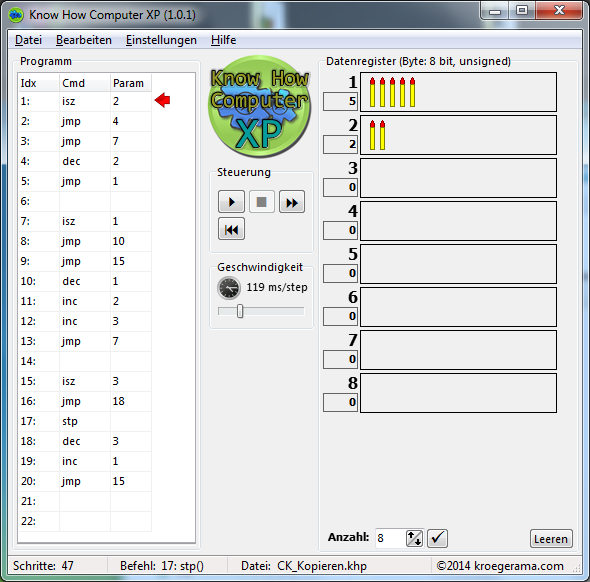
\includegraphics[width=0.8\textwidth]{9Diff-AB.III.3-Abb-1}
	\end{center}

	\begin{teilaufgaben}
		\teilaufgabe Gib nun in das Register 1 fünf Streichhölzer ein und in das Register 2
		zwei. Lass das Programm im \emph{Einzelschritt-Modus} ablaufen.

		\teilaufgabe Probiere andere Kombinationen an Werte in den Registern aus – auch
		welche, in denen Register 1 oder 2 leer sind.

		\teilaufgabe Beschreibe, was das Programm leistet.

		\teilaufgabe Zeichne für das Programm ein \emph{Ablaufdiagramm}.

		\teilaufgabe Erläutere nun, wie das Programm seine Aufgabe erledigt.

			{\hinweis{Das Programm besteht aus drei Blöcken: Zeile 1-5, Zeile 7-13
			und Zeile 15-20. Jeder Block ist für eine andere Teilaufgabe zuständig.}}

		\teilaufgabe\label{taufg:impl1} Verändere das Programm so, dass die Bedeutung von
		Register 1 und 2 vertauscht ist.

		\teilaufgabe\iconStern\ Verändere das Programm aus \ref{taufg:impl1} so, dass
		nach Beendigung des Programms Register 1 immer doppelt so viele Hölzer enthält,
		wie Register 2.
	\end{teilaufgaben}
\end{aufgabe}


\end{document}
